\section{Introduction} \label{sec:intro}


\begin{table}
\begin{tabular*}{\columnwidth}{|l|p{0.76\columnwidth}|}
\hline
\bf Symbol		& \bf Meaning \\\hline
$QR_{q,R}$		& Range query from $q$ to all $o_i : d_{q,o_i} < R$) \\\hline
$\chi_{s,t}$		& The frequency of a SP\\\hline
$P_{s,t}$		& A SP from s to t \\\hline
$d_{s,t}$		& The SP distance of a path $P_{s,t}$ \\\hline
$\mathfrak{d}_{s,t}$	& $\| t - s \|_2$, the euclidean distance \\\hline
$\mathcal{O}$		& The set of $POI \in \mathbf{V}$, the set of vertices\\\hline
$o_i$			& Element i in $\mathcal{O}$ \\\hline
$\mathcal{O}_{q,R}$	& The result set of  $o_i \in Q_{q,R}$ \\\hline
$dist_{\mathcal{O}}$	& Table of distances between vertexes $v_s, v_t \in P_{s,t} :  P_{s,t} \in SP_q$ \\\hline
$SP_{q}$		& A set of SP from q to all $o_i$ \\\hline
$\mathcal{QL_R}$	& Query log of range search queries \\\hline
$\Psi$ 			& The Cache \\\hline
$G\mathbf{(V,E)}$ 	& Graph representation of the Map \\\hline 

\end{tabular*}
\caption{Table of Symbols}
\label{tab:symbols}
\end{table}

\begin{algorithm}[bht]
\dontprintsemicolon
\SetVline

\SetKwInOut{Input}{input}\SetKwInOut{Output}{output}\SetKw{Return}{return}

\Input{

	$(q,R)$: A Range query\;
	$\mathcal{O}$: A set of POI \;
}

\Output{

	A set POI $\in \mathcal{O}$ \;
}

 \funcc{Naive}{(q,R), \mathcal{O}}
{
    \ForEach{$o_i \in \mathcal{O}$}
    {
      \If{$P_{q,o_i} \in \Psi$} 
      { 
	  $result \leftarrow P_{q,o_i}$ \;
      }
      \Else
      {
	  Calculate $P_{q,o_i}$ \tcp{\emph{SPfrom q to $o_i$}} \;
	  \If{$d_{q,o_i} \leq R$}  { $result \leftarrow o_i$ \; }
      }
    }
    \Return{result} \;
}

\caption{Naive Algorithm}
\label{alg:naive}
\end{algorithm}


\begin{algorithm}[bht]
\dontprintsemicolon
\SetVline

\SetKwInOut{Input}{input}\SetKwInOut{Output}{output}\SetKw{Return}{return}

\Input{

	$(q,R)$: A Range query\;
	$\mathcal{O}$: A set of POI \;
}

\Output{

	A set POI $\in \mathcal{O}$ \;
}

\funcc{Fair}{(q,R), \mathcal{O}}
{
    \ForEach{$o_i \in \mathcal{O} : \mathfrak{d}_{q,o_i} \leq R$}
    {
      $candidate_{\mathcal{O}} \leftarrow o_i$ \;
    }
     result $\leftarrow$ $candidate_{\mathcal{O}}$) \;

    \Return{result} \;
}

\caption{Fair Algorithm}
\label{alg:fair}
\end{algorithm}


\begin{align}\label{eq:chinaive}
\chi_{s,t}  = | \{P_{s,t}\} | :\; s \in QR_{s,R}, t \in \mathcal{O}, QR_{q,R} \in \mathcal{QL_R}
\end{align}

\begin{align}\label{eq:chifair}
\nonumber \chi_{s,t}  = | \{P_{s,t}\} |  :\; & \{ s \in QR_{s,R}, \{t \in \mathcal{O} | \mathfrak{d}_{s,t} \leq R \}, & \\
 & QR_{s,R} \in \mathcal{QL_R} \} &
\end{align}

\begin{definition}{Range Search}\\
A range search query, denoted by $Q_{q,R}$ consist of a source vertex $q$ and a range $\mathbf{R}$.
The result of $Q_{q,R}$, denoted $\mathcal{O}_{q,R}$, is a set of objects $o_i \in \mathcal{O}$ with SPdistance $d_{s,t} \leq R$ on graph $G\mathbf{(V,E)}$.
\end{definition}


\begin{definition}{Range Search Query Log ($\mathcal{QL_R}$)}\\
A range search query log $\mathcal{QL_R}$ is a collection of timestamped queries that have been issued by users in the past.
A query is on the form $(q,R)$, where $q$ is a query point and $R$ is a range. The full form of the log, $\mathcal{QL_R}$,  is then: $\{(q_0,R_0),\dots,(q_i,R_i)\}$
\end{definition}


Using a query log, $\mathcal{QL_R}: \{(q_0,R_0),\dots,(q_i,R_i)\}$, we first need to expand each query into its SPresult set containing SPs from $q$ to each POI reachable within R distance on a road network. 
To find the result set of a query we use one of two algorithms: \textbf{NAIVE} or \textbf{FAIR}ns.

The \textbf{NAIVE} algorithm will not only find the result set of SPfor each query $\in \mathcal{QL_R}$, but also the SPfrom $q$ to all other possible POIns, before pruning and returning the result set of POIsns.
\textbf{NAIVE} does so by first finding all paths from $q$ to any POI in the cache. Afterwards it will issue SPqueries from $q$ to the remaining POIs not already found via the cache. 
Once all paths are found \textbf{NAIVE} will prune the set of paths such that only the paths with distance < $R$ remain. This is the result so \textbf{NAIVE} returns it to the user.

The idea behind the \textbf{FAIR} algorithm (see alg. \ref{alg:fair}) is to prune POIsns, which can not belong to the result set of a query, before doing range search. The \textbf{FAIR} algorithm works by, for a query (q,R), first finding the set {\it tmpPOIns}, of POIs which lay within euclidean distance $R$ of the query point $q$. \textbf{FAIR} then invokes the \textbf{NAIVE} algorithm using {\it tmpPOIns} as the set of POIns.
The pruning method of \textbf{FAIR} is correct as the euclidean distance $R$ is also the longest SPns, with length $R$, possible. It is however important to note that this pruning technique only work if the weights of edges in a road network are distances.

Equation \ref{eq:chinaive} and \ref{eq:chifair} define the frequency of a SPin $\Psi$, using \textbf{NAIVE} or \textbf{FAIR} respectively.

An Example of how \textbf{FAIR} might work is shown in fig. \ref{fig:queryreg}. In it we have 2 queries: $q_1$ and $q_2$. Each query have a range $R=13$ associated with it, which is used to form the pruning areas (circles) of the queries. The pruning areas are the shown by the 2 circles, each covering a query. The  white circles are all vertices. $v_1,\ldots,v_{11}$ are the regular vertices. $o_1,\ldots,o_{10}$ represent the POIsns, and $q_1,q_2$ are the query points. Vertices ($\mathbf{V}$), and connecting lines,edges ($\mathbf{E}$), model a road network, $G\mathbf{(V,E)}$.

In our problem the range $R$ is constrained on a road network, meaning that after pruning, when the vertexes more than $R$ euclidean distance away are no longer considered, the remaining vertexes may still be further than $R$ distance in the road network. 
We can see an example of this with $q_2$, where only one out of the 3 POI in the gray region is actually within $R$ SPdistance ($o_9$, the reader should visually easily be able to confirm this using the edge weights in fig \ref{fig:queryreg}).

When we consider what to put into the cache, then we will include SPs for all POI within the pruning area, regardless of whether the POIs are contained in the result set or not. The reasoning behind this, is that if we only add the exact result, then we will not be able to determine if the entire result is in the cache or not, except in the special case that all vertexes in the pruning region is part of the result, as with query $q_1$.


\begin{figure}[hbt]
  \center
        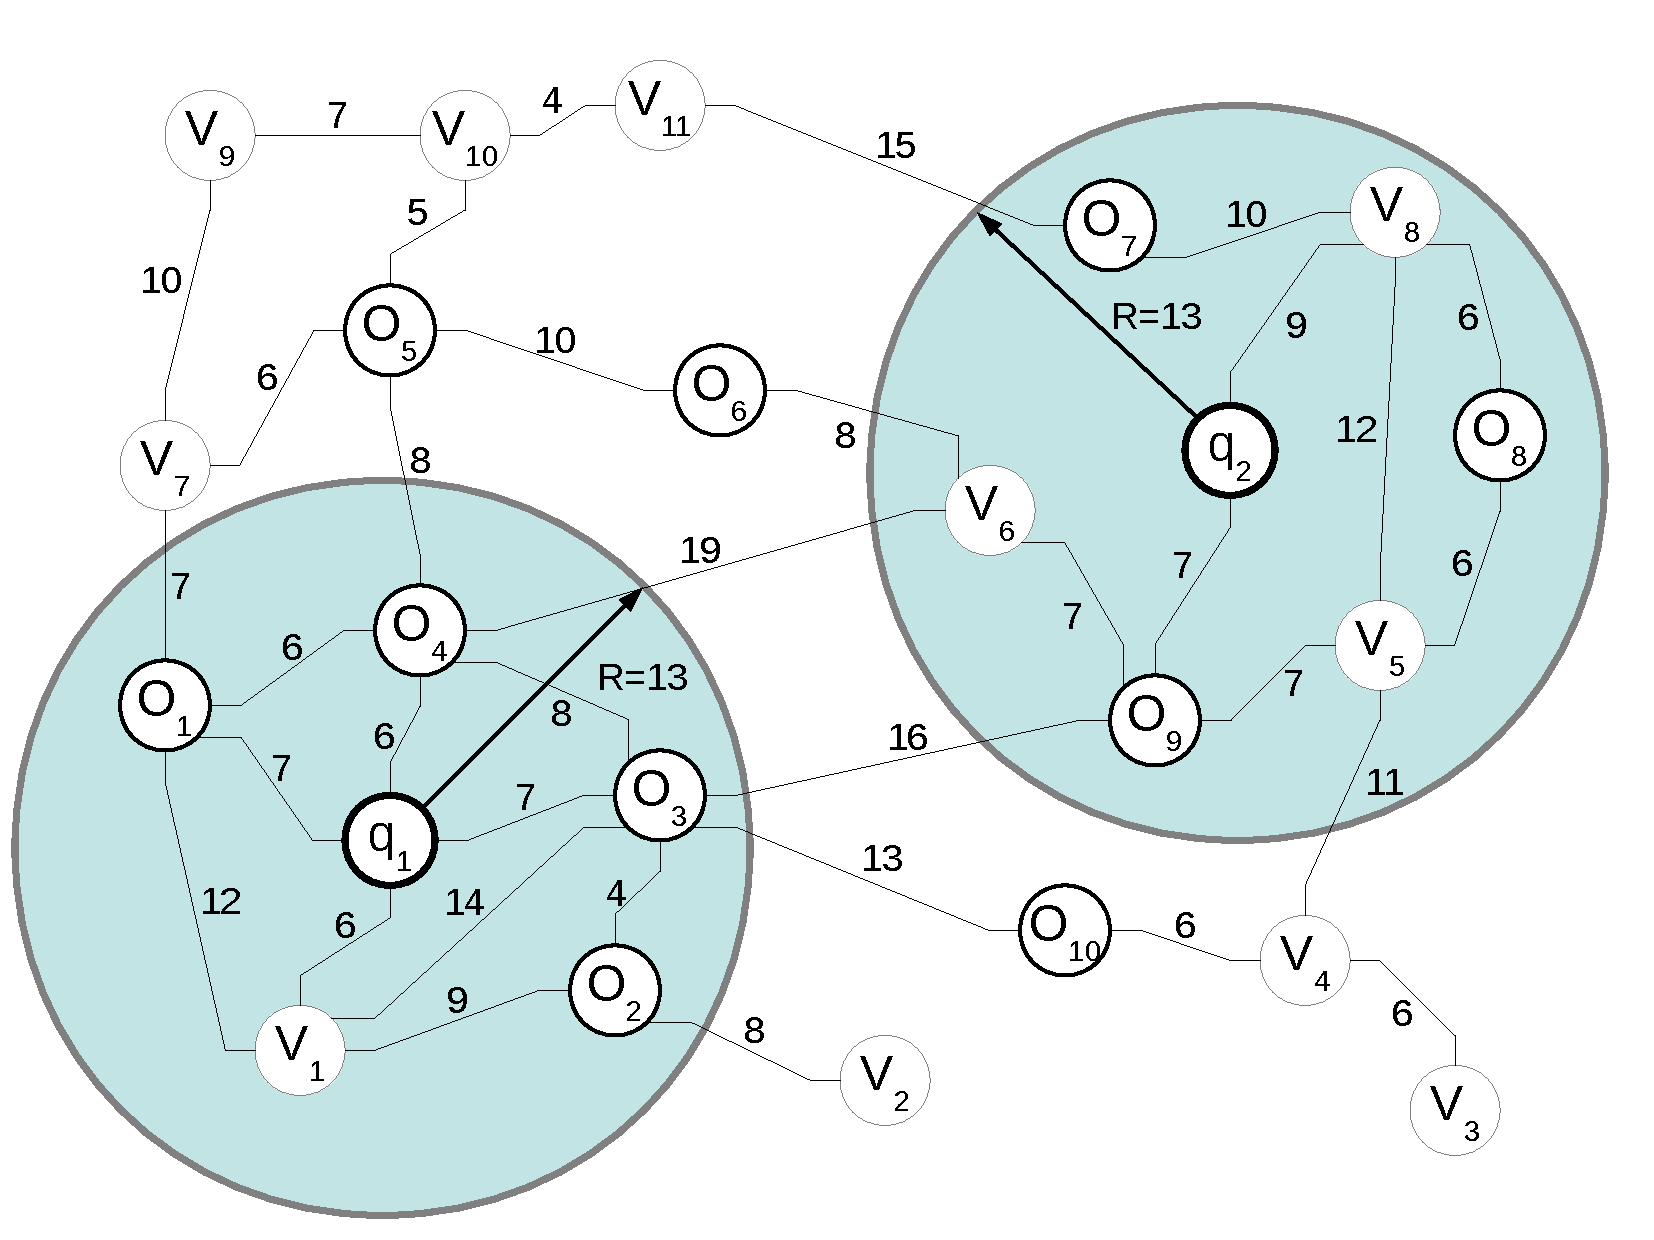
\includegraphics[width=0.5\textwidth]{figures/queryreg}
        \caption{Query points $q_1,q_2,q_3$, with region defined by R. White points are POIns}
  \label{fig:queryreg}
\end{figure}
